\documentclass[answers]{exam}

% ------------------------------------------------------------------------------ %
% -----------------------      Base for every .tex file   ---------------------- %
% ------------------------------------------------------------------------------ %

\usepackage[dvipsnames]{xcolor}
\usepackage{mathtools}
\usepackage{amssymb}
\usepackage{amsthm}
\usepackage{amsmath}
\usepackage{framed}
\usepackage{wasysym}
\usepackage{geometry}
\usepackage{cancel}
\usepackage{blindtext}
\usepackage{pgfplots}
\usepackage{graphicx}
\usepackage{lastpage}
\usepackage[most]{tcolorbox} 
\usepackage{multicol}
\usepackage{soul}
\usepackage{listings}
\usepackage{algorithm}
\usepackage{algorithmic}
\usepackage{booktabs}
\usepackage{tikz}
\usepackage{pifont}

% Libraries
\usetikzlibrary{shapes,shapes.geometric, positioning, arrows}

\geometry{%
	left=15mm,
	right=15mm,
	top=25mm,
	bottom=25mm,
	bindingoffset=0mm,
	headheight=30pt,% output from geometry tells you what this needs to be set to as a minimum
}

% Header and Footer
\pagestyle{headandfoot}
\firstpageheadrule
\runningheadrule
\firstpageheader{Convex Optimization}{\today}{Jonathan Schnell}
\runningheader{Convex Optimization}{}{Jonathan Schnell}
\firstpagefooter{}{Page \thepage\ of \numpages}{}
\runningfooter{}{Page \thepage\ of \numpages}{}

% Commands
\newcommand{\imp}[1]{\ul{\textbf{#1}}}
\newcommand{\dproduct}[1]{\left\langle #1 \right\rangle}
\newcommand{\norm}[1]{\left\lVert #1 \right\rVert}
\renewcommand{\vector}[1]{\begin{pmatrix} #1 \end{pmatrix}}
\newcommand{\abs}[1]{\left| #1 \right|}
\newcommand{\floor}[1]{\lfloor #1 \rfloor}
\newcommand{\ceil}[1]{\lceil #1 \rceil}
\newcommand{\fracpart}[2]{\frac{\partial #1}{\partial #2}}
\newcommand{\set}[2]{\left\{#1 \ \middle|\ #2\right\}}
\renewcommand{\hat}[1]{\widehat{#1}}

\newcommand{\Ker}{\operatorname{Ker}}
\renewcommand{\Im}{\operatorname{Im}}
\renewcommand{\Re}{\operatorname{Re}}
\renewcommand{\dim}{\operatorname{dim}}
\renewcommand{\div}{\operatorname{div}}
\newcommand{\rot}{\operatorname{rot}}
\newcommand{\grad}{\operatorname{grad}}
\newcommand{\vol}{\operatorname{vol}}
\newcommand{\supp}{\operatorname{supp}}
\renewcommand{\div}{\operatorname{div}}
\newcommand*{\vertbar}{\rule[-1ex]{0.5pt}{2.5ex}}
\newcommand*{\horzbar}{\rule[.5ex]{2.5ex}{0.5pt}}

\theoremstyle{definition}
\newtheorem*{definition}{Definition}
\newtheorem*{beispiel}{Beispiel}
\newtheorem*{remark}{Remark}

\theoremstyle{plain}
\newtheorem*{proposition}{Proposition}
\newtheorem*{satz}{Satz}
\newtheorem*{korollar}{Korollar}
\newtheorem*{lemma}{Lemma}
\newtheorem*{theorem}{Theorem}


% Quote
\newtcolorbox{zitat}[1]{%
	colback=lightGray,
	grow to right by=-10mm,
	grow to left by=-10mm, 
	boxrule=0pt,
	boxsep=0pt,
	breakable,
	enhanced jigsaw,
	borderline west={4pt}{0pt}{gray},
	#1
}

% Use colors in equations
\newcommand{\highlight}[2]{\colorbox{#1}{$#2$}}%
\definecolor{lightGray}{gray}{0.9} 

% To add shortcut of script Letters in Equations
\newcommand{\s}[1]{\mathcal{#1}}
\newcommand*\circled[1]{\tikz[baseline=(char.base)]{
            \node[shape=circle,draw,inner sep=2pt] (char) {#1};}}
\newcommand{\cmark}{\ding{51}}
\newcommand{\xmark}{\ding{55}}


\newenvironment{claim}[1]{
		\par\noindent
		\textbf{Claim.} #1
		\begin{tcolorbox}[blanker, top=3mm, bottom=3mm, left=3mm, borderline west={1pt}{0mm}{black}]
		\noindent\textit{Proof of Claim.} 
}{
	\hfill$\blacksquare$	
	\end{tcolorbox}\noindent
}

% To add shortcut of number's set Z
\newcommand*{\Z}{\mathbb{Z}}
\newcommand*{\N}{\mathbb{N}}
\newcommand*{\R}{\mathbb{R}}
\newcommand*{\Q}{\mathbb{Q}}
\newcommand*{\C}{\mathbb{C}}
\newcommand*{\F}{\mathbb{F}}
\newcommand*{\K}{\mathbb{K}}

% To add shortcut of empty set
\renewcommand*{\o}{\varnothing}
\pgfplotsset{compat=1.9}

\everymath{\displaystyle}

% Line-Height
\linespread{1.15}

\graphicspath{{Files/}}

% ------------------------------

\begin{document}

	$ $
	\begin{center}
		\huge \textbf{Exercise session notes - Week 3}  \\ \vspace*{3mm}
        \Large{Convex Functions}
	\end{center}
	$ $\\
    
    \paragraph*{Definitions.} A function $f:X\to \R$ is convex if $X$ is convex and one of the following (equivalent) conditions hold:\vspace{5mm} \\ 
    \begin{minipage}{12cm}
        \begin{itemize}
            \item $0$th-order characterization: for any $x,y\in X$ and $\lambda\in [0,1]$ we have 
            $$ f(\lambda x + (1-\lambda)y)\leq \lambda f(x) + (1-\lambda)f(y) $$
            Meaning: the line between any two points in the graph of $f$ lies above the function $f$. 
        \end{itemize} 
    \end{minipage}
    \hspace*{3mm}
    \begin{minipage}{6cm}    
        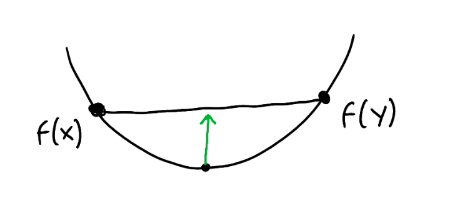
\includegraphics[width=\textwidth]{0thConvex.PNG}
    \end{minipage} \vspace*{5mm} \\ 
    \begin{minipage}{12cm}
        \begin{itemize}
            \item $1$st-order characterization: for any $x,y\in X$ we have 
            $$ f(y)\geq f(x) + \nabla f(x)^\top(y-x) $$
            Meaning: the function $f$ entirely lies above the first order taylor approximation at each point $x$.
        \end{itemize} 
    \end{minipage}
    \hspace*{3mm}
    \begin{minipage}{6cm}    
        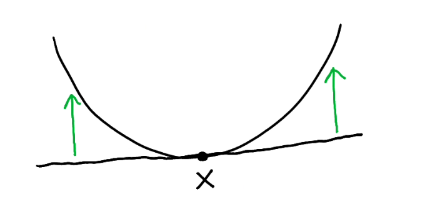
\includegraphics[width=\textwidth]{1stConvex.PNG}
    \end{minipage} \vspace*{5mm} \\ 
    \begin{minipage}{12cm}
        \begin{itemize}
            \item $2$nd-order characterization: for any $x\in X$ we have 
            \begin{align*}
                &\ \nabla^2 f(x)\text{ is Positive Semi Definite} \\ 
                \iff&\ v^\top\cdot  \nabla^2 f(x)\cdot v \geq 0 \quad\quad \forall v\in \R^n
            \end{align*}
            $$ $$
            Meaning: the curvature of the function $f$ is positive (the function $f$ is "trying to go upwards").
        \end{itemize} 
    \end{minipage}
    \hspace*{3mm}
    \begin{minipage}{6cm}    
        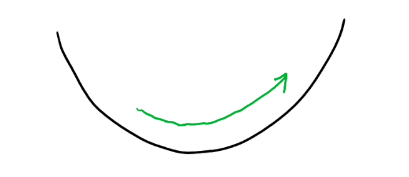
\includegraphics[width=\textwidth]{2ndConvex.PNG}
    \end{minipage} \clearpage
    \paragraph{Examples.} Here are some examples of important convex/concave functions. \vspace*{2mm}
    \begin{center}\renewcommand{\arraystretch}{1.7}
        \begin{tabular}{p{7cm}cp{7cm}}
            Convex Functions. & $\qquad\longleftrightarrow\qquad$ & Concave Functions\\ 
            \cmidrule{1-1}\cmidrule{3-3}
            Affine $ax+ b$ for $a,b\in \R$ &  & Affine $ax+ b$ for $a,b\in \R$ \\ 
            Exponentials $e^{ax}$ for $a\in \R$ & & Logarithms $\log_a(x)$ for $a \geq 1$ \\
            Powers $x^a$ in $\R_{>0}$ for $a\leq 0$ or $a\geq 1$ & & Powers $x^a$ in $\R_{>0}$ for $a\in [0,1]$ \\
            Any norm $\norm{x}_p = \left(\sum \abs{x_i}^p\right)^{1/p}$ for $p\in [1,\infty]$ & &  \\
            LogSumExp $\log\left(e^{x_1}+\cdots + e^{x_n}\right)$.\newline 
            $\hookrightarrow$ This is a smooth approximator of the max funcion. & &
        \end{tabular}
    \end{center}
    \paragraph*{Properties.} Here are some operations that preserve convexity.
    \begin{itemize}
        \item Sums (conic combinations) $\sum a_i f_i$ for $a_i\geq 0$ \newline
        In particular $f_1 + f_2$ is convex.
        \item Affine Precompositions. If $f$ convex then $f(Ax + b)$ is convex. \newline
        E.g. $\norm{Ax + b}$ is convex (Norm approximation error)
        \item If $f(x,y)$ convex in $x$ then $g(x) := \sup_{y}f(x,y)$ is convex.\newline
        E.g. Max eigenvalue of symmetric matrix $\lambda_{max}(A) = \sup_{\norm{y}=1}y^\top A y$
        \item If $f$ convex + non-decreasing and $g$ convex then $f\circ g$ convex. \newline
        E.g. If $g$ convex then $e^{g(x)}$ convex
        \item If $f$ convex + non-increasing and $g$ concave then $f\circ g$ convex.\newline
        E.g. If $g$ concave+positive then $1/g(x)$ convex.
    \end{itemize}
\end{document}